\documentclass[border=6pt]{standalone}
\usepackage{tikz}
\usetikzlibrary{arrows.meta,positioning,fit,calc}
\definecolor{fg}{HTML}{DBC9A8}
\definecolor{fgbody}{HTML}{C4A882}
\definecolor{stroke}{HTML}{C4963C}
\definecolor{surf}{HTML}{22222B}
\definecolor{surfemph}{HTML}{2A2820}
\definecolor{surfact}{HTML}{2E2020}
\definecolor{bdim}{HTML}{9A7F62}
\definecolor{bemph}{HTML}{D4A849}
\definecolor{bact}{HTML}{FF5C5C}
\begin{document}
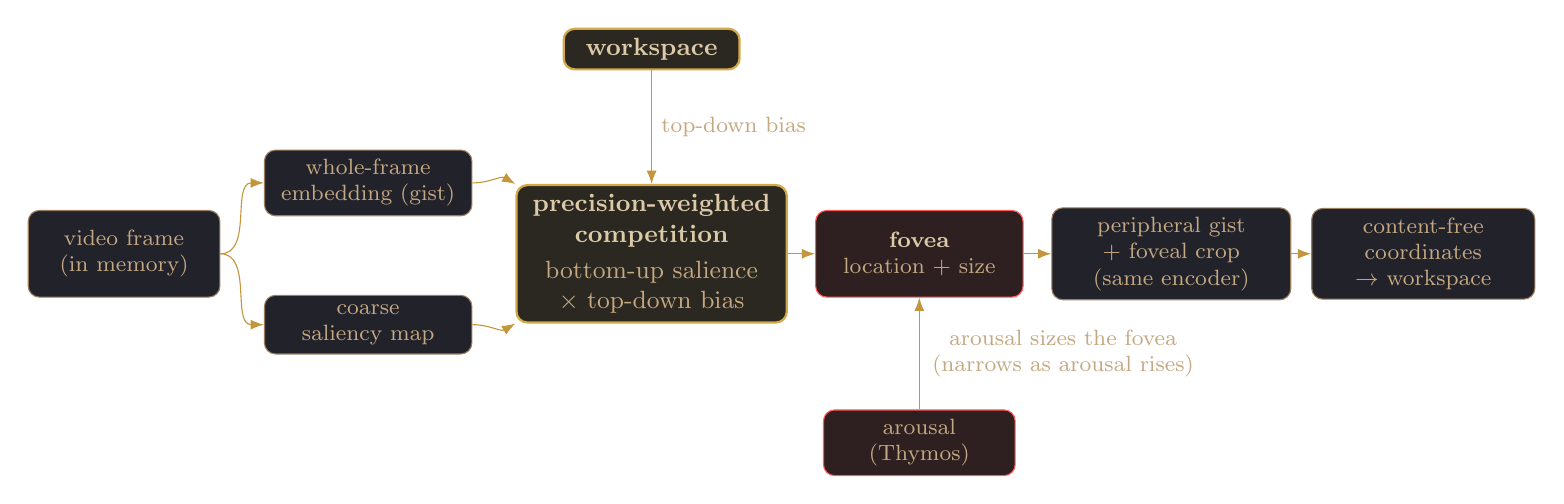
\begin{tikzpicture}[
  font=\small,>=Latex,
  every node/.append style={text=fgbody},
  mod/.style={draw=bdim, rounded corners, fill=surf, align=center, font=\footnotesize},
  work/.style={draw=bemph, thick, rounded corners, fill=surfemph, align=center},
  act/.style={draw=bact, rounded corners, fill=surfact, align=center, font=\footnotesize},
  lbl/.style={font=\footnotesize, text=fgbody, align=center},
]
% main vision flow (left -> right)
\node[mod, text width=22mm, minimum height=11mm] (cam) at (0,0) {video frame\\(in memory)};
\node[mod, text width=24mm] (emb) at (3.1,0.9) {whole-frame embedding (gist)};
\node[mod, text width=24mm] (sal) at (3.1,-0.9) {coarse saliency map};
\node[work, text width=32mm, minimum height=14mm] (comp) at (6.7,0)
  {\textcolor{fg}{\textbf{precision-weighted competition}}\\[2pt]bottom-up salience $\times$ top-down bias};
\node[act, text width=24mm, minimum height=11mm] (fov) at (10.1,0)
  {\textcolor{fg}{\textbf{fovea}}\\location $+$ size};
\node[mod, text width=28mm] (crop) at (13.3,0) {peripheral gist $+$ foveal crop (same encoder)};
\node[mod, text width=26mm] (coord) at (16.5,0) {content-free coordinates $\rightarrow$ workspace};
% top-down source
\node[work, text width=20mm] (wsn) at (6.7,2.6) {\textcolor{fg}{\textbf{workspace}}};
% arousal source
\node[act, text width=22mm] (ar) at (10.1,-2.4) {arousal (Thymos)};
% flows
\draw[->, draw=stroke] (cam.east) to[out=0,in=180] (emb.west);
\draw[->, draw=stroke] (cam.east) to[out=0,in=180] (sal.west);
\draw[->, draw=stroke] (emb.east) to[out=0,in=150] (comp.north west);
\draw[->, draw=stroke] (sal.east) to[out=0,in=210] (comp.south west);
\draw[->, draw=stroke] (comp.east) -- (fov.west);
\draw[->, draw=stroke] (fov.east) -- (crop.west);
\draw[->, draw=stroke] (crop.east) -- (coord.west);
\draw[->, draw=stroke] (wsn.south) -- node[lbl, right]{top-down bias} (comp.north);
\draw[->, draw=stroke] (ar.north) --
  node[lbl, right, text width=34mm]{arousal sizes the fovea (narrows as arousal rises)} (fov.south);
\end{tikzpicture}
\end{document}
